\documentclass[acmtog]{techreportacmart}

\usepackage{booktabs} % For formal tables
\usepackage{physics}
\usepackage{subcaption}

\usepackage[ruled]{algorithm2e} % For algorithms
\renewcommand{\algorithmcfname}{ALGORITHM}
\SetAlFnt{\small}
\SetAlCapFnt{\small}
\SetAlCapNameFnt{\small}
\SetAlCapHSkip{0pt}
\IncMargin{-\parindent}

% Copyright
\setcopyright{none}

\settopmatter{printacmref=false, printccs=false, printfolios=true}
\citestyle{acmauthoryear}
\setcitestyle{square}

% Document starts
\begin{document}
% Title portion
\title{A Short Report on Learning to Control PDEs With Differentiable Physics} 
\author{Barnab\'{a}s B\"{o}rcs\"{o}k}
\affiliation{%
  \institution{Technical University of Munich}
}
\author{Lukas Prantl}
\affiliation{
  Advisor,
  \institution{Technical University of Munich}
}

\renewcommand\shortauthors{Barnab\'{a}s B\"{o}rcs\"{o}k}

\begin{abstract}
  Modelling, understanding and controlling the physical world around us is
  a longstanding problem in many disciplines. Partial Differential Equations
  (PDEs) are one of the most general and popular way of describing evolving
  physical systems. We phrase the problem as applying external forces to our
  system in order to reach a predefined end state after given time steps, with
  the control force being as small as possible. We do this by leveraging
  differentiable physics for the optimization problem. The method presented 
  trains two neural network actors for the distinct tasks of predicting an
  optimal route between the predefined states and finding the necessary minimal
  control forces: a predictor-corrector scheme.

  We base this short report on the work and results of \cite{ControlPDEs}. 

  Although the methods presented are general enough to handle any types of
  mathematical models governed by PDEs, the current work discusses its use for
  physical simulations, such as fluid simulation. 
\end{abstract}

\keywords{Physical Simulations, Partial Differential Equations, Differentiable
Physics}


\thanks{This report is a part of the lecture, Master-Seminar -- Deep Learning in
  Physics, Informatics 15, Technical University of Munich.\\

The original work is introduced by \cite{ControlPDEs}.\\

A supplementary result of \cite{ControlPDEs} was $\Phi_{Flow}$, an open-source
simulation toolkit written mostly in Python. It is available at 
\url{https://github.com/tum-pbs/PhiFlow}. All of the figures were in this report
were generated with $\Phi_{Flow}$, based on the official examples provided. 
}

\maketitle

\section{Introduction}
In this section, we will give a brief overview of notation, and techniques
necessary to understand the following techniques.

\section{Problem}
Given a physical system $\vb{u}(\vb{x}, t)$, whose natural evolution is
described by the PDE
\begin{equation}
  \label{eq:problem-pde}
  \pdv{\vb{u}}{t} = 
  \mathcal{P} \left( 
    \vb{u},
    \pdv{u}{x},
    \pdv[2]{u}{x},
    \dots,
    \vb{y}(t)
  \right),
\end{equation}

$\mathcal{P}$ models the physical behavior of the system, and $\vb{y}(t)$
denotes external factors that can influence the system. We introduce an agent
into our system that is able to exert force on the system, thus modifying it.
This can be for example a wind blowing over a body of water, or induced by an
electric motor. We factor out all these influences into a force term
$\vb{F}(t)$, that influences $\mathcal{P}$ over time:

\begin{equation}
  \label{eq:problem-pde}
  \pdv{\vb{u}}{t} = 
  \mathcal{P} \left( 
    \vb{u},
    \pdv{u}{x},
    \pdv[2]{u}{x},
    \dots
  \right) +
  \vb{F}(t).
\end{equation}

We can now model the agent as a function that computes $\vb{F}(t)$.

In most real-world scenarios, it is not possible to observe the full state of
a physical system. Considering a cloud of smoke, for example, we might be able
to observe the density field, but the velocity may not be observable directly.
We model this imperfect information by defining the observable state of $\vb{u}$
as $\vb{o}(\vb{u})$. All of these are problem dependent. Our agent is
conditioned only on these observations, which means it does not have access to
the full state $\vb{u}$. 

Note that the differentiable solver still has access to the full state,
otherwise the simulation could not be executed properly. When deploying the
trained agent to the real world, the simulation is replaced by real world
physics, but the trained models can still infer the control forces, as they
depend only on the observation of these states. 


Given an initial observable state $\vb{o}(t_0) = \vb{o_0}$ and a target state
at time $\vb{o}(t_*) = \vb{o}_*$, we would like to match these at time $t_0$ and
$t_*$:
\begin{equation}
\begin{split}
  \label{eq:problem-loss-match-state}
  \vb{o}(\vb{u}(t_0)) &= \vb{o_0} \\ 
  \vb{o}(\vb{u}(t_*)) &= \vb{o_*}
\end{split}
\end{equation}

We would also like to minimize the amount of force applied within the
simulation domain $\mathcal{D}$:
\begin{equation}
  \label{eq:problem-loss-force}
  L_{\vb{F}}\left[ \vb{u}(t) \right] = 
  \int_{t_0}^{t_*}
    \int_{\mathcal{D}} \left| \vb{F}_{\vb{u}}(t)\right|^2  \dd{x}
  \dd{t}
\end{equation}

In practice, we usually take discrete time steps $\Delta t$ to approximate these
integrals, in which case the trajectory $\vb{u}$ is a sequence of $n = (t_*
- t_0)/\Delta t$ states.

We can combine our expectations defined in
Equations~\eqref{eq:problem-loss-match-state}~and~\eqref{eq:problem-loss-force}
into the loss function
\begin{equation}
  \label{eq:loss-function}
  L[\vb{u}(t)] = \alpha \cdot L_{\vb{F}}[\vb{u}(t)] + 
  L_o^*(\vb{u}(t_*)),
\end{equation}

with $\alpha > 0$. $L_o^*(\vb{u}(t_*))$ is the observation loss, in place to
make sure that we match the states in
Equation~\eqref{eq:problem-loss-match-state} as closely as we can. There may not
always exist a trajectory $\vb{u}(t)$ that matches both $\vb{o_0}$ and
$\vb{o_*}$. This can happen due to many things, such as physical constraints, or
numerical limitations. 

We use square brackets to denote functions that depend on fields or sequences
rather than single values. These are also called functionals. 

\section{Preliminaries}

\subsection{Differentiable Solvers}
% Read preliminaries -> differentiable physics
The target is to minimize a differentiable physics loss function. 
A differentiable solver is used to compute the forward physics and the
corresponding gradients to optimize for the loss function. 

Let $\vb{u}(\vb{x}, t)$ be described by the PDE $\mathcal{P}$ as in
Equation~\eqref{eq:problem-pde}. A regular solver can step the system forward in
time via Euler steps:
\begin{equation}
  \vb{u}(t_{i+1}) = Solver[\vb{u}(t_i), \vb{y}(t_i)] =
  \vb{u}(t_i) + \Delta t \cdot \mathcal{P}(\vb{u}(t_i), \dots, \vb{y}(t_i)),
\end{equation}

moving the system forward in time by $\Delta t$. Repeated execution integrates
us a trajectory $u(t)$, approximating a solution to the PDE. This functionality
is not enough by itself to solve optimization problems, as the derivatives
needed can only be acquired using finite differences, giving us numerical
derivates that are neither efficient nor reliable for the computation of
derivatives. 

Differentiable solvers improve upon this by giving us analytic derivatives.
A differentiable solver can efficiently compute the derivatives with respect to
any of its inputs, i.e. 
\[
\delta \vb{u}(t_{i+1}) / \delta \vb{u}(t_i) 
\text{ or } 
\delta \vb{u}(t_{i+1}) / \delta \vb{y}(t_i). 
\]
We can utilize this functionality for our gradient-based optimization of either
inputs or control parameters over an arbitrary number of time steps. 

\subsection{Iterative trajectory optimization}
When trying to estimate a control force $\vb{F}(t)$, it is common to start out
with a random value, and iteratively improve upon it, until reaching an optimum.
The simplest of these techniques is known as single shooting: one optimization
step consists of simulating the full dynamics, and then backpropagating the loss
through the whole sequence to optimize the control forces. For a sequence of $n$
frames, this means having $n$ copies of the estimator. We call such an agent
a control force estimator (CFE), whose task is to find an optimal force
$\vb{F}(t)$.

After backpropagating through the whole series, the weight updates are
accumulated from each copy of the CFE. 

Optimizing a chain of CFEs as described above is both computationally expensive,
and potentially yields unstable gradients. The latter is a problem especially
when the initialization is far off from an optimum, giving unstable $\Delta u$
gradients. This is usually the case at the beginning of the optimization.

Differentiable physics losses solve these problems by allowing the agent to be
directly optimized for the desired objective function. 
% \textbf{QUESTION TO ADVISOR: This means that all of the linked CFEs are updated
% after each Adjoint solve, and they share the same weights?} 

When backpropagating the gradients through the whole sequence, the differentiable
solver backpropagates the gradients through the simulation. The main benefit of
using a differentiable physics solver is that it has feedback on how its
decisions change the future trajectory as well as how to handle states as input
that were reached because of its previous decisions. As there is no ground truth
needed, problems with multiple possible solutions will naturally converge
towards one solution. This is also illustrated on the toy example presented in 
Figure~\ref{fig:learning-to-throw}.

% \textbf{QUESTION TO ADVISOR: How do physics losses achieve these advancements
% over the single-shooting method? Why did the paper illustrate the
% Single-shooting optimization instead of what they use? Is the illustration the
% same for the employed differentiable solver?}

\begin{figure*}
  \centering
  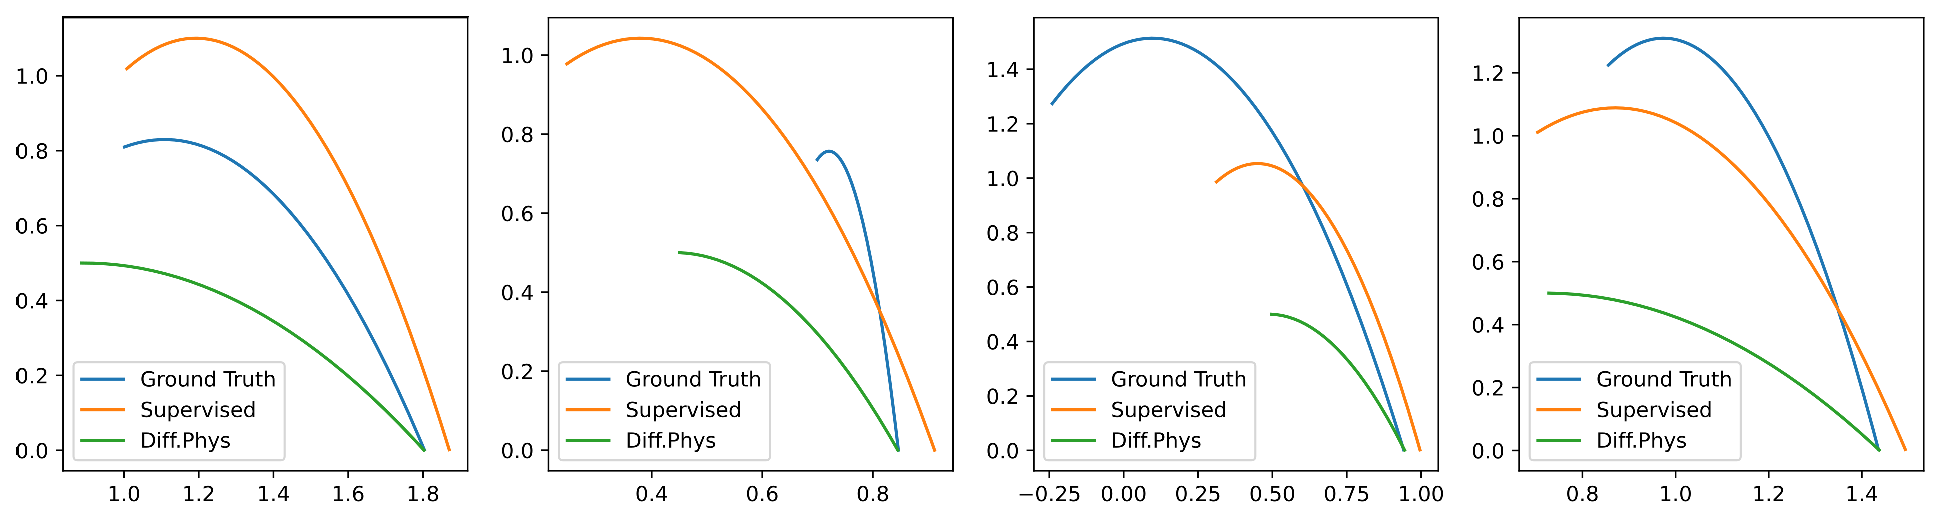
\includegraphics[width=0.8\textwidth]{throwing_results}
  \caption{Learning to throw. 
    An example, showcasing an important difference between supervised and
    differentiable physics approaches. Both the supervised and the differentiable physics
    network approximate the function $f^{-1}(\vb{x_{final}}): \mathbb{R} \mapsto
    \mathbb{R}^4$, which is the inverse of the function $f(\vb{x}, \vb{y},
    \vb{v}, \vb{\alpha})$, mapping the final position $\vb{x_{final}}$ of an
    object being thrown from position $(\vb{x}, \vb{y})$, with velocity $\vb{v}$
    and angle $\vb{\alpha}$. The same network architecture is used, with the
    weights initialized to the same initial values. Both networks have seen the
    same number of training examples, and are using an $L_2$ norm between the
    point of impact resulting from the predicted initial values and the intended
    position. It is evident that the DP network is able to get orders of
    magnitude closer than the supervised network, which has no knowledge of the
    underlying physical system, and it's best guess is to interpolate between
    the closest data it has seen during training, which results in a coarse
    approximation. Also, as the result space to this problem is not unimodal
    (e.g. it has multiple possible right answers), the supervised model
    is further thrown off, and will give values in-between. This means that even
    if we increase the training data, our supervised model can never learn this
    problem properly.
  }
  \label{fig:learning-to-throw}
\end{figure*}

\section{Method}

In order to successfully interact with the physical system, the agent has to 
\begin{itemize}
  \item build an internal representation of an optimal observable trajectory
    $\vb{o}(\vb{u}(t))$ and
  \item learn what actions to take in order to move the system along this
    trajectory.
\end{itemize}

\cite{ControlPDEs} separate these two subtasks into a predictor-corrector
scheme, that given an $\vb{o}(t)$ computes $\vb{o}(t + \Delta t)$  in two steps.
First, a predicted $\vb{o}^p(t+\Delta t)$ is given, which is then corrected to
yield $\vb{o}(t+\Delta t)$. These steps can be mostly learned independently.
This motivates us to separate these tasks into two distinct agents, trained
independently.

First, an observation predictor (OP) predicts the next observation state, given
the current one: $\vb{o}_{t+1}^p(\vb{o}_t)$ for all time steps, giving us
$\vb{o}_i, i \in {1,2,\dots, n-1}$. Then, a control force estimator (CFE)
predicts $\vb{F}(t_i |\vb{o}(\vb{u}_i), o^p_{i+1} )$, the force necessary to
move the simulation to the predicted next state as close as possible.

Once this $\vb{F}(t)$ force is estimated up until a time step $n$, an
opportunity is presented to update the simulation until time step $n$, which in
turn makes it possible to predict a trajectory that more closely resembles the
actual evolution of $\vb{u}$. 

\cite{ControlPDEs} generalize the OP agent to predict not directly the state
$\vb{o}^p(t_{i+1} | \vb{o}(\vb{u}_i), \vb{o}^*)$, but instead to predict the
optimal center point between two states at times 
$i, j \in {1,2,\dots,n-1}, j > i$, given the observed states at these times: 
$\vb{o}^p((t_i + t_j)/2 | \vb{o}_i, \vb{o}_j)$. Modeling OP in this way lends
itself to recursively evaluating partitions, until a prediction $\vb{o}^p(t_i)$
for every time step $t_i$ has been made, starting with 
$\vb{o}^p((t_0 + t_*)/2 | \vb{o}_0, \vb{o}_*)$.

This separation has the added benefit of exposing the predicted path between the
initial and end states. As physical systems can often demonstrate different
behaviors on different time scales, and the OP can be called with arbitrary two
time steps, we will train multiple distinct instances of OPs for each time
scale we need. This does not add a significant overhead and also simplifies
training. We will refer to OPs trained for different timescale as OP$_n$ for the
number of frames $n = (t_j - t_i)/ \Delta t$.

\subsection{Execution order} 
Considering the different possible orders in which we can execute the OP and CFE
predictions gives us multiple options regarding the order of execution. The most
straight-forward ordering is \textit{prediction first}: first predicting the
observed states $\vb{o}_{t_i}$ for every time step between $t_0$ and $t_*$, starting
with the half-way point $\vb{o}_{t_{n/2} | \vb{o}_0, \vb{o}_*}$, predicted by OP$_n$.
After predicting all observed states, we can evaluate the actual path: for each
time step, we train the CFE to get $\vb{F}(t_i|\vb{o}(\vb{u}_i,
\vb{o}_{i+1}^p))$, and stepping the simulation forward after each call to the
CFE. The main problem with this set-up is that sometimes the reconstructured
trajectory from OPs can only be matched partially due to either physical
constraints or numerical inaccuracies. When subsequent predictions do not align,
and the deviation between the predicted and calculated observations deviate too
much, the CFE might apply too large forces, resulting in undesirable jitters or
even not following the predicted trajectory altogether.

This problem is preventable by using \textit{staggered execution}, where an OP
is trained only when its corresponding start frame has been calculated by the
CFE, thus being able to take the deviations into account between the actual
evolution $\vb{o}(\vb{u}(t))$ and the prediction $\vb{o}^p(t)$.

Although \textit{staggered execution} is already an improvement upon
\textit{prediction first}, some of the predicted observations remain unchanged
throughout training, most notably the observation 
$\vb{o}_{n/2 | \vb{o}_0, \vb{o}_*}$, halfway between the start frame $t_0$ and
end frame $t_*$. When the simulation reaches such point, there might be
a deviation big enough to justify refining the prediction for this point based
on the actual evolution of $\vb{u}(t)$.  The
\textit{prediction refinement} algorithm is introduced to alleviate these
problems. For further discussion and illustrations on the different execution
orders, please refer to \cite{ControlPDEs}.

\subsection{Architecture and training}
\cite{ControlPDEs} use a modified U-Net architecture \cite{unet}, a typical
multi-level convolutional network architecture with skip connections. They
modify the basic architecture by using residual blocks \cite{residual-blocks}.
A more detailed description of the architecture is given in Appendix~C of the
original paper.

The networks were implemented in Tensorflow \cite{tensorflow} and trained using
the ADAM optimizer on an Nvidia GTX 1080 Ti. Batch sizes ranging from 4 to 16
were used.

Supervised training usually converged within a fraction of the first epoch, so
supervised training was stopped after a few epochs, comprising between $2000$
and $10.000$ iterations.

Training with the differentiable solver was significantly slower, since the
backpropagation through long chains is more challenging than training with
a supervised loss. Optimization steps are also considerably more expensive since
the whole chain needs to be executed, including the forward and the backward
simulation pass. For the 2D fluid examples, a single optimization step took 1-2
seconds to complete. The training for the examples shown took between one and
two days. 

\section{Results}
\cite{ControlPDEs} evaluate the capabilities of their method to learn to control
PDEs in three different environments of increasing complexity.
\subsection{Burger's Equation}
Burger's Equation is a nonlinear PDE describing the time evolution of a single
field $u$. Following Equation~\eqref{eq:problem-pde}, it can be written as
\begin{equation}
  \mathcal{P} \left( 
    u, \pdv{u}{x}, \pdv[2]{u}{x},
  \right) = 
  -u \cdot \pdv{u}{x} + \nu \pdv[2]{u}{x}.
\end{equation}

The full state was observable, e.g. $o(u) = u$

\cite{ControlPDEs} analyze the results both qualitatively and quantitatively.
Even though the CFE scheme requires only 1/200th the inference time, it does not
manage to converge to the ground truth, while the supervised and differentiable
physics losses manage to approximate the expected evolution of $u$, the
differentiable physics version giving much smoother results. 

\subsection{Incompressible fluid flow}
The Navier-Stokes equations govern incompressible fluid flows. For a velocity
field $\vb{v}$, these can be written as
\begin{equation}
    \mathcal{P} \left( 
      \vb{v}, \nabla \vb{v}
    \right) = 
    -(\vb{v}\times \nabla)\vb{v} + \nu \nabla^2\vb{v} - \frac{\nabla p}{\rho_f}
\end{equation}
subject to the hard constraints $\nabla \cdot \vb{v}= 0$ and  $\nabla \times p = 0$,
where $p$ denotes pressure and $\nu$ the viscosity. A constant fluid density is
assumed throughout the simulation, setting $\rho_f = 1$.

\cite{ControlPDEs} train the OP and CFE networks for two different tasks:
\begin{itemize}
  \item reconstruction of natural fluid flows
  \item controlled shape transitions
\end{itemize}

\cite{ControlPDEs} used $128^2$ grids, with the ability to apply forces
to the whole of $\vb{v}$, resulting in more than $16.000$ continuous control
parameters. Additionally, a passive density $\rho$ is added that
moves with the fluid via $\pdv{\rho}{t} = -\vb{v} \cdot \nabla \rho$. $\vb{v}$
is set to be hidden, and $\rho$ to be observable. 

A reduced example of controlling shape transitions is shown in
Figure~\ref{fig:shape-transition}

\begin{figure*}
  \centering
  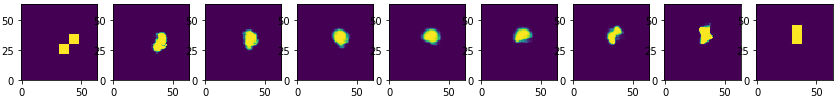
\includegraphics[width=1.0\textwidth]{shape-transition.png}
  \caption{
    An example of training the network for shape transition, advancing from the
    initial state $\vb{o_0}$ to the desired state $\vb{o_*}$ through some
    reconstructed states $\vb{o}(u(t_i))$ from left to right. This example was
    created using a $64 \times 64$ grid. 
  }
  \label{fig:shape-transition}
\end{figure*}

\subsection{Incompressible fluid with indirect control}
The most complicated setup has an increased complexity due to adding obstacles
to the simulated domain and also limiting the area that can be controlled by the
network. As before, only the density $\rho$ is observable. Here, the goal is to
move the "smoke" from its original position into a predefined "bucket" at the
top of the domain, as seen in
Figures~\ref{fig:indirect-a}~through~\ref{fig:indirect-c}.

\subsubsection{Simulation Control}
As mentioned previously, controlling the world around us is a long-standing
problem in many disciplines beyond the study of fluid simulations, like
robotics or environmental engineering, with numerous real life applications.

In an overview talk\footnote{https://youtu.be/BwuRTpTR2Rg}, the authors compared
the discussed indirect control problem to a fire breaking out in a room, and
having to blow the fire out by controlling the ventilation system around the
room. 

\begin{figure}
  \label{fig:indirect}
  \centering
  \begin{subfigure}{0.15\textwidth}
    \centering
    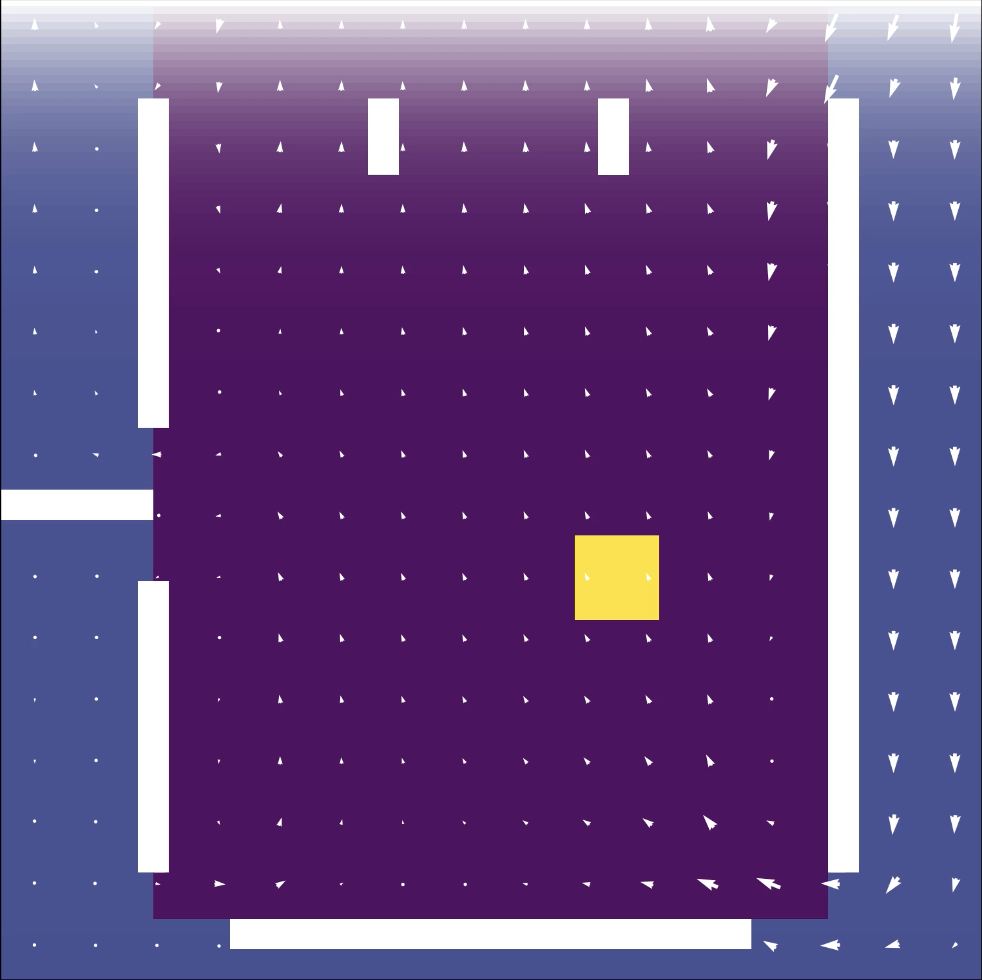
\includegraphics[width=\textwidth]{indirect_start.png}
    \caption{start}
    \label{fig:indirect-a}
  \end{subfigure}
  \begin{subfigure}{0.15\textwidth}
    \centering
    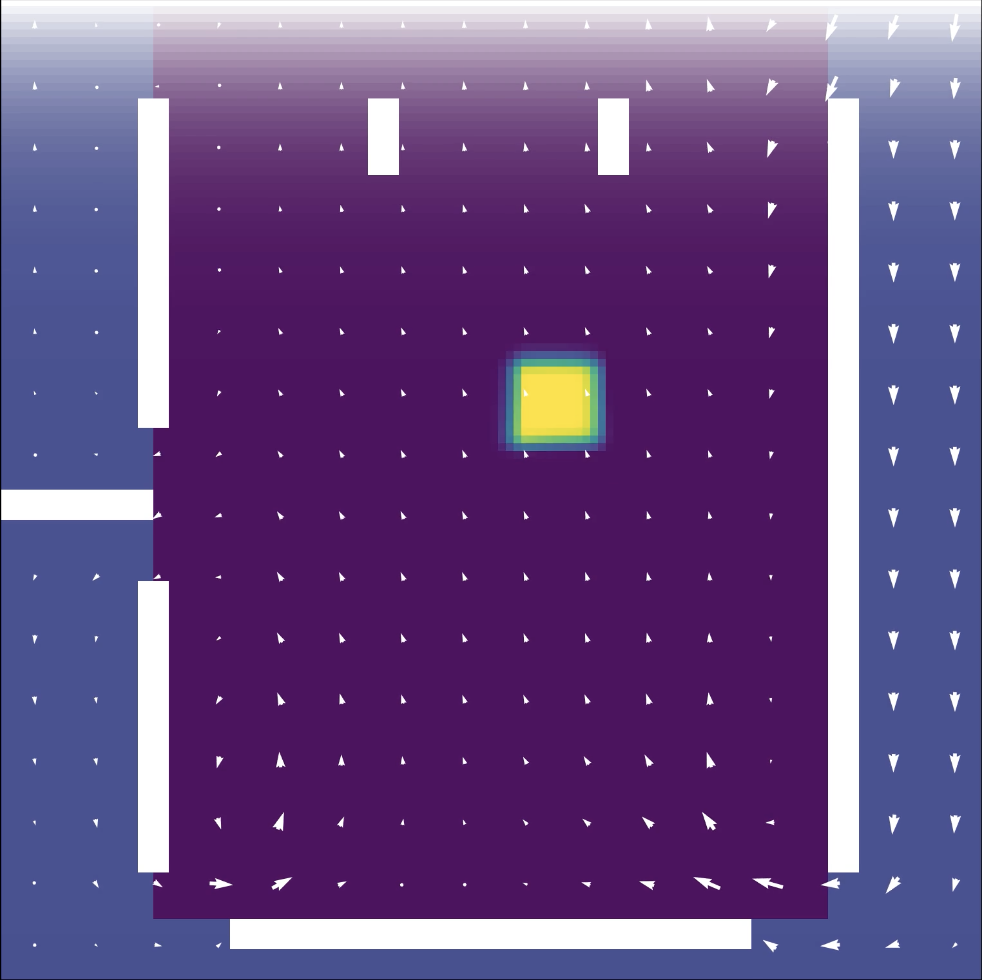
\includegraphics[width=\textwidth]{indirect_middle.png}
    \caption{}
    \label{fig:indirect-b}
  \end{subfigure}
  \begin{subfigure}{0.15\textwidth}
    \centering
    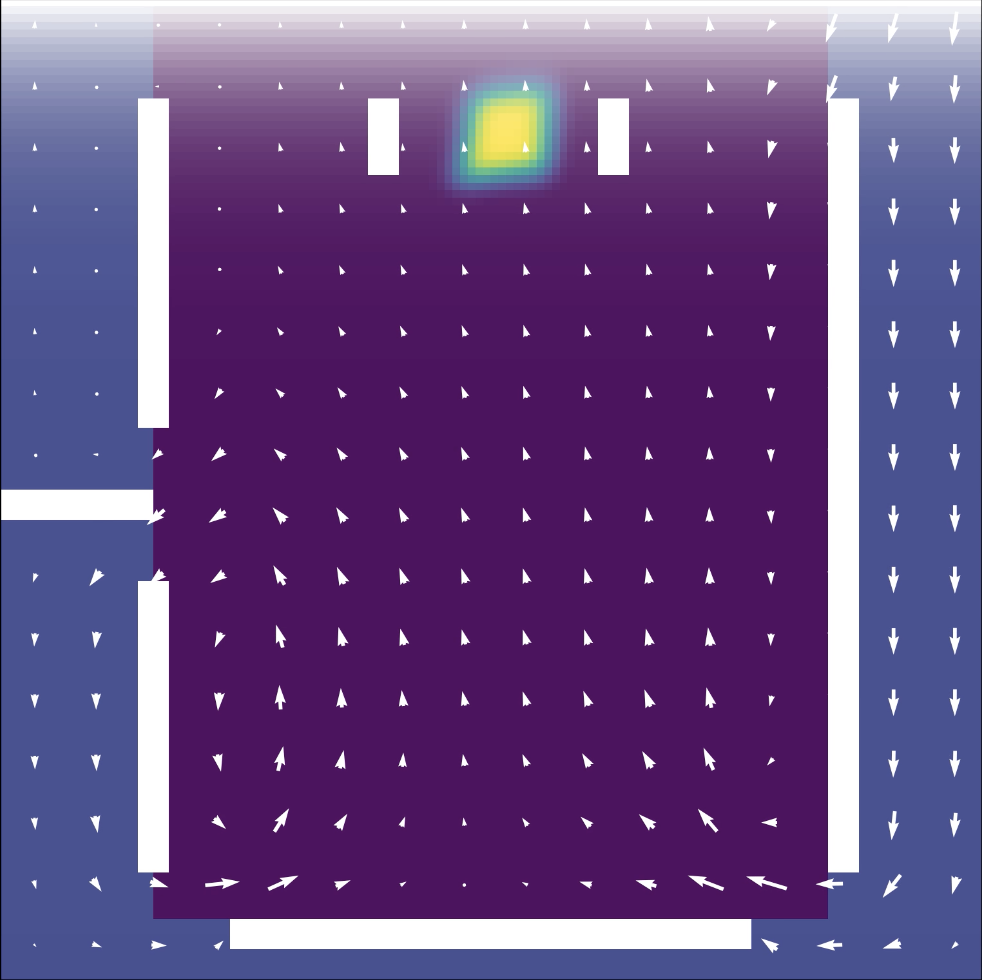
\includegraphics[width=\textwidth]{indirect_end.png}
    \caption{end}
    \label{fig:indirect-c}
  \end{subfigure}
  \caption{Incompressible fluid with indirect control. The agent is able to
  exert force in the blue region, and is able to observ the density $\rho$,
  denoted with yellow. The objective is to get all of the material out on
  a predefined "bucket"}
\end{figure}

\subsection{Source}
All results are accessible in online form as supplemental materials,\footnote{https://ge.in.tum.de/download/2020-iclr-holl/supplemental/supplemental.html}
as well as in the Appendices of the original paper.

The code for recreating the discussed results is also available.
\footnote{https://github.com/holl-/PDE-Control}

\subsection{Comparison with Existing Methods}
\cite{ControlPDEs} compare their method with multiple baselines both
analitically and quantitatively. In their experiments, using prediction
refinement with differentiable physics training yields the best results. 

% \section{Outlook -- Discussion}
% The mathematical basis for approximating functions of (almost) arbitrary
% complexity with Neural Networks (NNs) has been around for a long time now.
% Owing to recent technological advancements, especially in GPU
% technology, the long-standing goal of using NNs for real-life
% problems is starting to come to a reality. 

% Although gradient-based learning has been used since the late 1950's, they were
% mostly limited to linear systems.\cite{Duda1973PatternCA}
% Kickstarted in big part by \cite{6795724} and \cite{726791}, followed by the
% introduction of Convolutional Neural Networks (CNNs)
% \cite{cnn}, NNs and CNNs are currently heavily used, from predicting protein
% structures \cite{AlphaFold2021}, to learning to play complex games such
% as StarCraft \cite{starcraft} or Go \cite{go} expertly. Due to these
% advancements in use cases, NNs and Deep Learning systems are sometimes being
% referred to as \textit{Artifical Intelligence} or \textit{AI} systems. The
% notion of these agents being \textit{intelligent} beyond approximating
% functions in a usually predefined form can be misleading for the general public. 
% Even if the input is a matrix of RGB values, and the output array of values can
% be interpreted in a meaningful way besides a numerical answer, at the heart, NNs
% are still approximating mathematical functions: they take numbers in, and give
% numbers out.

% \subsection{Neural Networks are Universal Function Approximators}
% The paper by \cite{ControlPDEs} highlights this explicitly, training the agents
% to approximate the function $\vb{F}(t)$ as in Equation~\eqref{eq:problem-pde}.
% The idea of using pre-existing knowledge and methods, while inserting a new
% \textit{NN module} into these solutions, to gain both the benefit of speed from
% NNs, as well as the explainability and predictability from existing models, has
% a wide range of applicability. 

% An example of enhancing the speed of an existing method by leveraging NNs
% is also given by \cite{DeepScatter}. They reached a $24\times$ faster
% convergence for cloud rendering by training a NN to approximate the indirect
% in-scattered radiance function for Monte Carlo integration.

\section{Conclusion}

\cite{ControlPDEs} introduce a novel method to control PDEs with differentiable
physics: a hierarchical corrector-predictor scheme, dividing the problem into
easier subproblems. The proposed method was applied to solve different
challenging PDEs, such as the 1D Burger's equation, and the Navier-Stokes
equations (in 2D) to tackle incompressible fluid flow problems.

The approach has possible applications far beyond the examples used for
illustrating the method. Controlling systems governed by PDEs, such as robotics,
environmental engineering, or describing wildlife populations.

\begin{acks}

  The author would like to thank Lukas Prantl for advising the report, the other
  organizers of the Master-Seminar -- Deep Learning in Physics of the 2022
  Summer semester, as well as the original authors of the paper discussed.

\end{acks}

% Bibliography
\bibliographystyle{ACM-Reference-Format}
\bibliography{bibliography}

\end{document}
